\documentclass{beamer}

\mode<presentation>
{
  \usetheme{Warsaw}
  \setbeamercovered{transparent}
}
\usepackage[english]{babel}
\usepackage[utf8]{inputenc}
\usepackage{times}
\usepackage{float}
\usepackage[T1]{fontenc}

\title[PROYECTO - ANDROID] 
{S E A R C H --- S A V E}


\subtitle{}
\institute[ESCUELA SUPERIOR]
{	
	\centering
  		
\includegraphics[totalheight=1in,width=1in]{ss}
  		
	ESCUELA SUPERIOR\\
	POLITECNICA DEL LITORAL
}
\date[CFP 2012]{Proyecto en Android, 2012}

\begin{document}
	\begin{frame}
  	  \titlepage
	\end{frame}
	
	%Integrantes del Grupo
	\begin{frame}{INTEGRANTES}
		 \begin{flushleft}
 			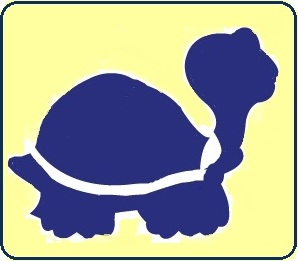
\includegraphics[totalheight=1.2in,width=2in]{LTwitspol}
 		 \end{flushleft}
 		 
 		 \begin{itemize}
 		 	\item
 		 		\begin{flushright}
 		 			Cuadrado Daniel
 		 		\end{flushright}
 		 	\item
 		 		\begin{flushright}
 		 			Mite Juan 
 		 		\end{flushright}
 		 	\item
				\begin{flushright} 		 		
 		 		Torres Criollo Daniel
 		 		\end{flushright}
 		 	\item
 		 		\begin{flushright}
 		 			Velez Gomez José
 		 		\end{flushright}
 		 \end{itemize}
  	\end{frame}
  	  	
  	%Seccion Introduccion
  	\begin{frame}{DESCRIPCION DE LA APLICACION}
  		\centering
  		
\includegraphics[totalheight=1in,width=1in]{ss}	
  		\begin{block}{}
  		La aplicación pasa mayor parte del tiempo ejecutándose en segundo plano, cuando el usuario ingresa tema de consulta la guarda, si el teléfono tiene acceso a internet la aplicación busca la pagina (HTML) encontrada con el tema especifico y la convierte en un formato PDF y  la almacena en la micro SD.
  		\end{block}				
	\end{frame}
	
	\begin{frame}{FUNCIONALIDADES DE LA APLICACION}
		\centering
  		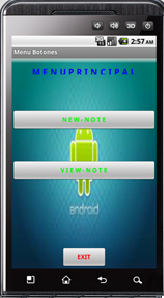
\includegraphics[totalheight=1.4in,width=0.9in]{menu}
  		\begin{block}{}
  		La aplicación SEARCH-SAVE fue ideada para resolver el problema que tienen ciertos usuarios, que es el de olvidar palabras o temas de consulta que escucha en la vida cotidiana y los cuales siente curiosidad, pero que en ese momento esta imposibilitado para hacer dicha consulta.
  		\end{block}				
	\end{frame}
	
	\begin{frame}{A QUIEN VA DIRIGIDA LA APLICACION}
		\centering
  		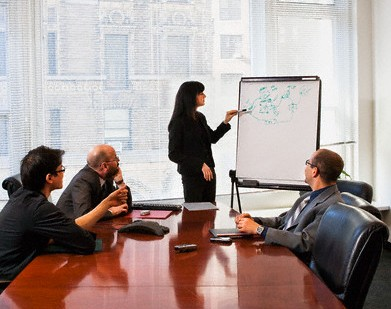
\includegraphics[totalheight=1in,width=1.5in]{meeting}	
  		\begin{block}{}
  		Esta aplicación está dirigida a las personas que no todo el tiempo disponen de internet en su teléfono.
  		\end{block}				
	\end{frame}
	

	\begin{frame}{EJECUTANDO LA APLICACION}
		\centering
  		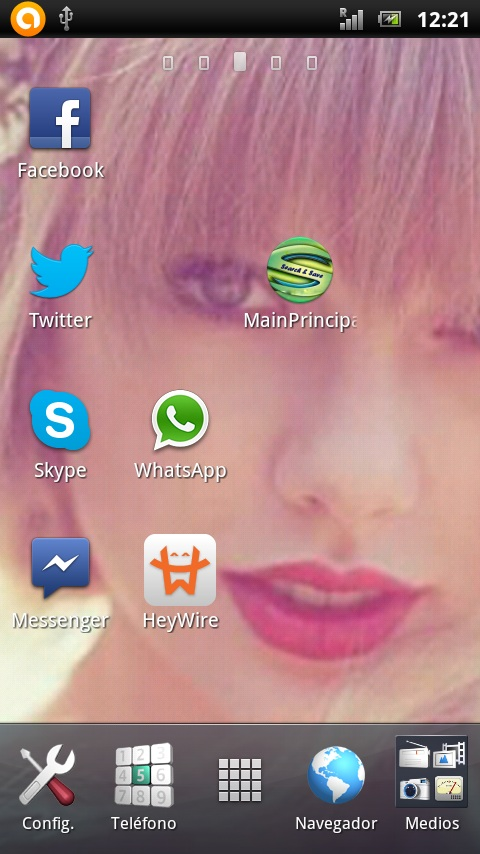
\includegraphics[totalheight=2in,width=1.5in]{menuand}	
  		\begin{block}{}
  		Luego de diseñar la interfaz de la aplicación, en el menú principal de Android podemos observar el logo de "Search and Save".
		\end{block}
	\end{frame}

	\begin{frame}{EJECUTANDO LA APLICACION}
		\centering
  		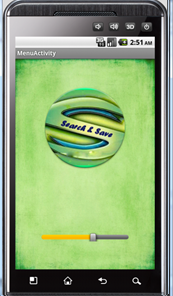
\includegraphics[totalheight=2in,width=1.5in]{cargando}
  		\begin{block}{}
  		Cargando la aplicacion.
  		\end{block}
 	\end{frame}

	\begin{frame}{EJECUTANDO LA APLICACION}
		\centering
  		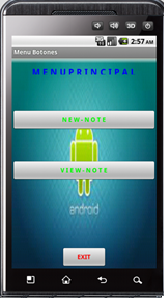
\includegraphics[totalheight=2in,width=1.5in]{menuapp}	
  		\begin{block}{}
  		Menu de la aplicacion.
  		\end{block}
 	\end{frame}
 	\begin{frame}{EJECUTANDO LA APLICACION}
		\centering
  		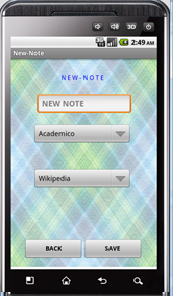
\includegraphics[totalheight=2in,width=1.5in]{notas}
  		\begin{block}{}
  		Abriendo New Note.
  		\end{block}	
 	\end{frame}
 	
 	\begin{frame}{EJECUTANDO LA APLICACION}
		\centering
  		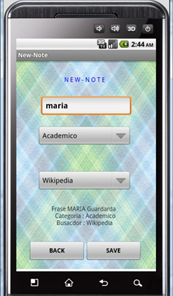
\includegraphics[totalheight=2in,width=1.5in]{ingresarnota}	
  		\begin{block}{}
  		Guaradando una frase.
  		\end{block}
 	\end{frame}

\begin{frame}{EJECUTANDO LA APLICACION}
		\centering
  		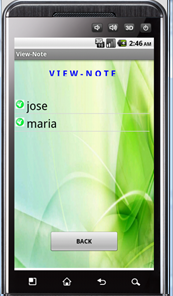
\includegraphics[totalheight=2in,width=1.5in]{vernotas}	
  		\begin{block}{}
  		Lista guardada.
  		\end{block}
 	\end{frame}
	%\appendix	
	%\section<presentation>*{\appendixname}
	\subsection<presentation>*{SEARCH-SAVE -- ANDROID}
	\begin{frame}
	\centering
		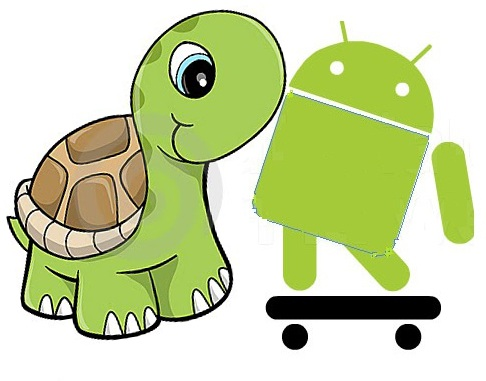
\includegraphics[width=0.3\textwidth]{Android}
		
		\begin{center}
			M U C H A S \\ G R A C I A S 
		\end{center}
	\end{frame}
	
	
\end{document}

